\section*{Problem 2: Tries}


\noindent
\textbf{a)} Zeichnen Sie einen unkomprimierten und einen komprimierten Trie für die Wörter \{ALGORITHMUS, TRIE, BAUM, TORUS, BAHN, TORPEDO\}.\\



\textbf{Aufgabe 2a:} 
\textbf{unkomprimierter Trie:}
\begin{center}
    \textbf{1. insert(ALGORITHMUS)}
\end{center}
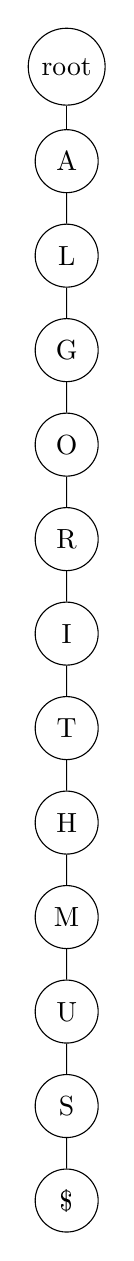
\begin{tikzpicture}[
  level distance=1.2cm,
  every node/.style={draw, circle, minimum size=0.8cm}
]


\node {root}
  child {node {A}
    child {node {L}
      child {node {G}
        child {node {O}
          child {node {R}
            child {node {I}
              child {node {T}
                child {node {H}
                  child {node {M}
                    child {node {U}
                      child {node {S}
                        child {node {\$}}
                      }
                    }
                  }
                }
              }
            }
          }
        }
      }
    }
  };
\end{tikzpicture}

\newpage

\begin{center}
    \textbf{2. insert(TRIE)}
\end{center}
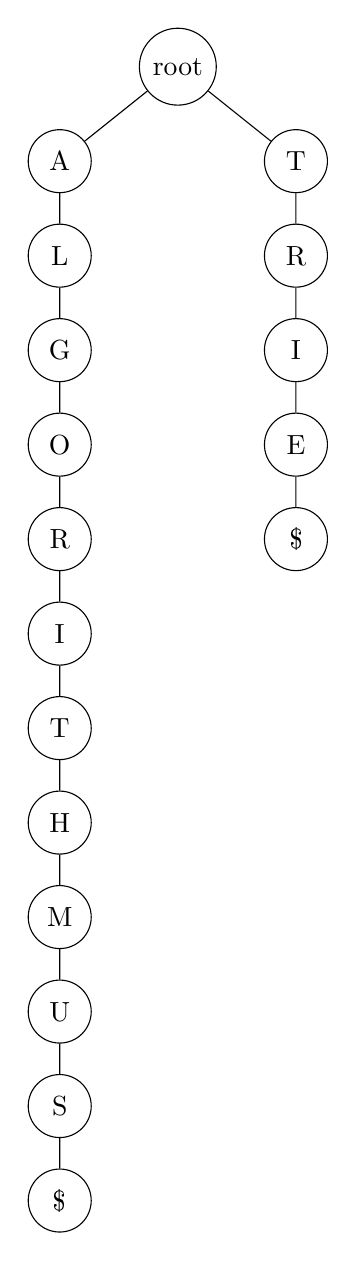
\begin{tikzpicture}[
  level distance=1.2cm,
  level 1/.style={sibling distance=3cm},
  every node/.style={draw, circle, minimum size=0.8cm}
]

\node {root}
  child {node {A}
    child {node {L}
      child {node {G}
        child {node {O}
          child {node {R}
            child {node {I}
              child {node {T}
                child {node {H}
                  child {node {M}
                    child {node {U}
                      child {node {S}
                        child {node {\$}}
                      }
                    }
                  }
                }
              }
            }
          }
        }
      }
    }
  }
  child {node {T}
    child {node {R}
      child {node {I}
        child {node {E}
          child {node {\$}}
        }
      }
    }
  };
\end{tikzpicture}

\newpage

\begin{center}
    \textbf{3. insert(BAUM)}
\end{center}
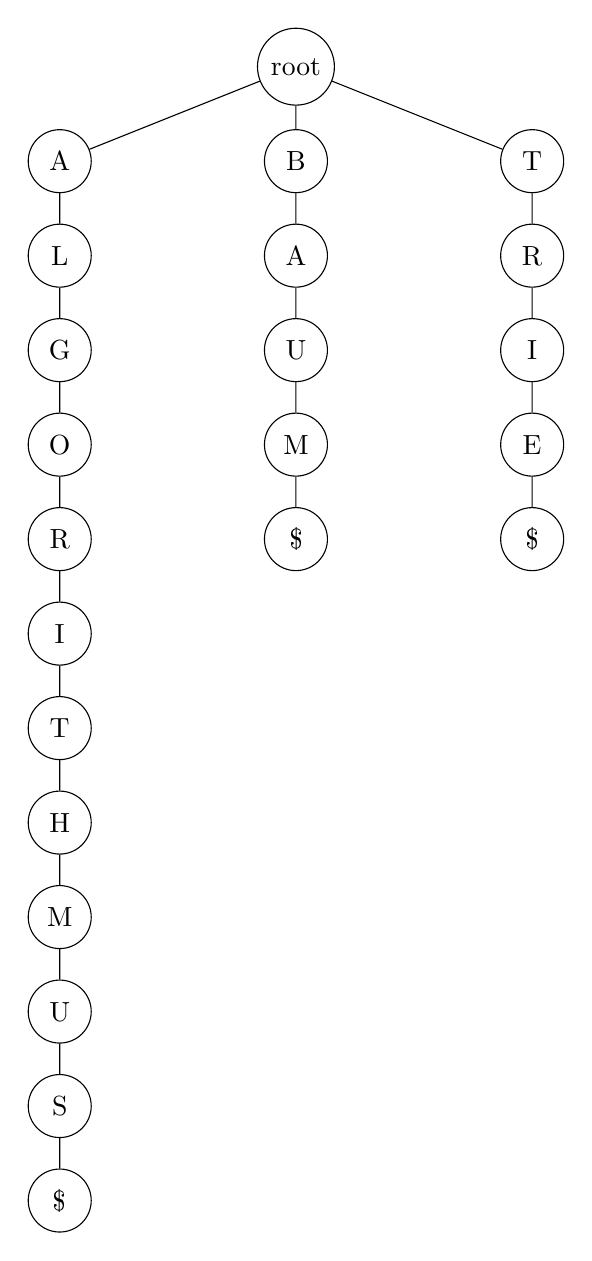
\begin{tikzpicture}[
  level distance=1.2cm,
  level 1/.style={sibling distance=3cm},
  level 2/.style={sibling distance=1.5cm},
  every node/.style={draw, circle, minimum size=0.8cm}
]

\node {root}
  child {node {A}
    child {node {L}
      child {node {G}
        child {node {O}
          child {node {R}
            child {node {I}
              child {node {T}
                child {node {H}
                  child {node {M}
                    child {node {U}
                      child {node {S}
                        child {node {\$}}
                      }
                    }
                  }
                }
              }
            }
          }
        }
      }
    }
  }
  child {node {B}
    child {node {A}
      child {node {U}
        child {node {M}
          child {node {\$}}
        }
      }
    }
  }
  child {node {T}
    child {node {R}
      child {node {I}
        child {node {E}
          child {node {\$}}
        }
      }
    }
  };
\end{tikzpicture}

\newpage

\begin{center}
    \textbf{4. insert(TORUS)}
\end{center}
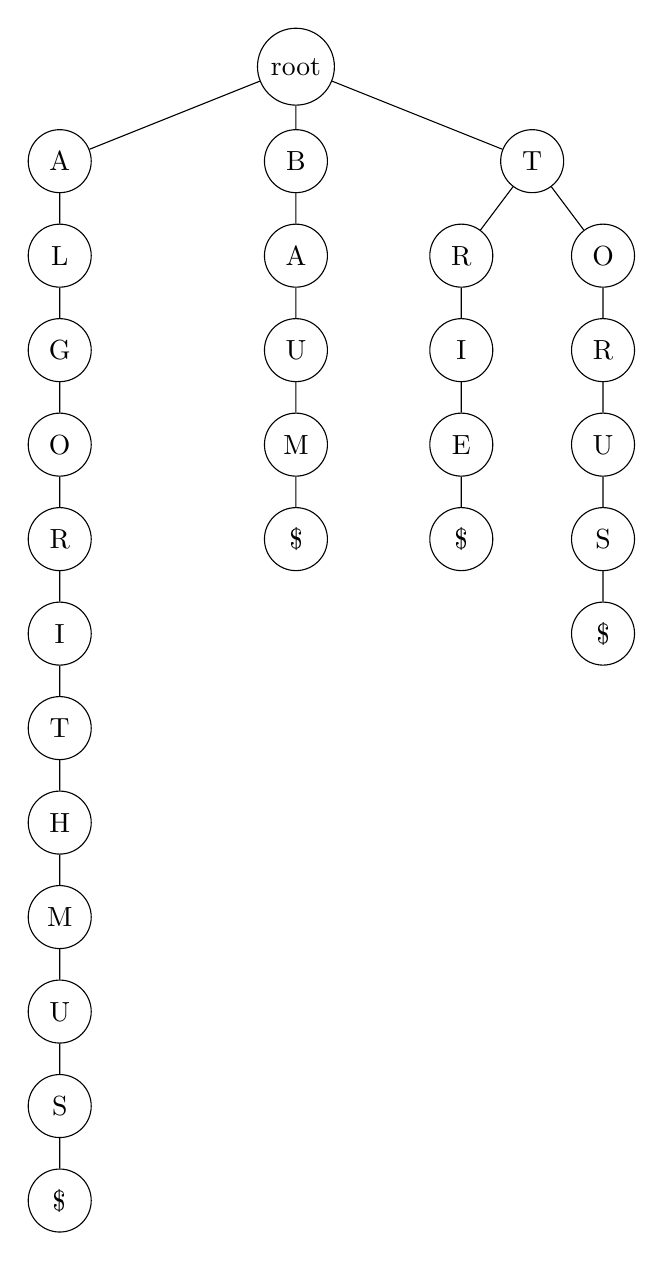
\begin{tikzpicture}[
  level distance=1.2cm,
  level 1/.style={sibling distance=3cm},
  level 2/.style={sibling distance=1.8cm},
  level 3/.style={sibling distance=1.5cm},
  every node/.style={draw, circle, minimum size=0.8cm}
]

\node {root}
  child {node {A}
    child {node {L}
      child {node {G}
        child {node {O}
          child {node {R}
            child {node {I}
              child {node {T}
                child {node {H}
                  child {node {M}
                    child {node {U}
                      child {node {S}
                        child {node {\$}}
                      }
                    }
                  }
                }
              }
            }
          }
        }
      }
    }
  }
  child {node {B}
    child {node {A}
      child {node {U}
        child {node {M}
          child {node {\$}}
        }
      }
    }
  }
  child {node {T}
    child {node {R}
      child {node {I}
        child {node {E}
          child {node {\$}}
        }
      }
    }
    child {node {O}
      child {node {R}
        child {node {U}
          child {node {S}
            child {node {\$}}
          }
        }
      }
    }
  };
\end{tikzpicture}

\newpage

\begin{center}
    \textbf{5. insert(BAHN)}
\end{center}
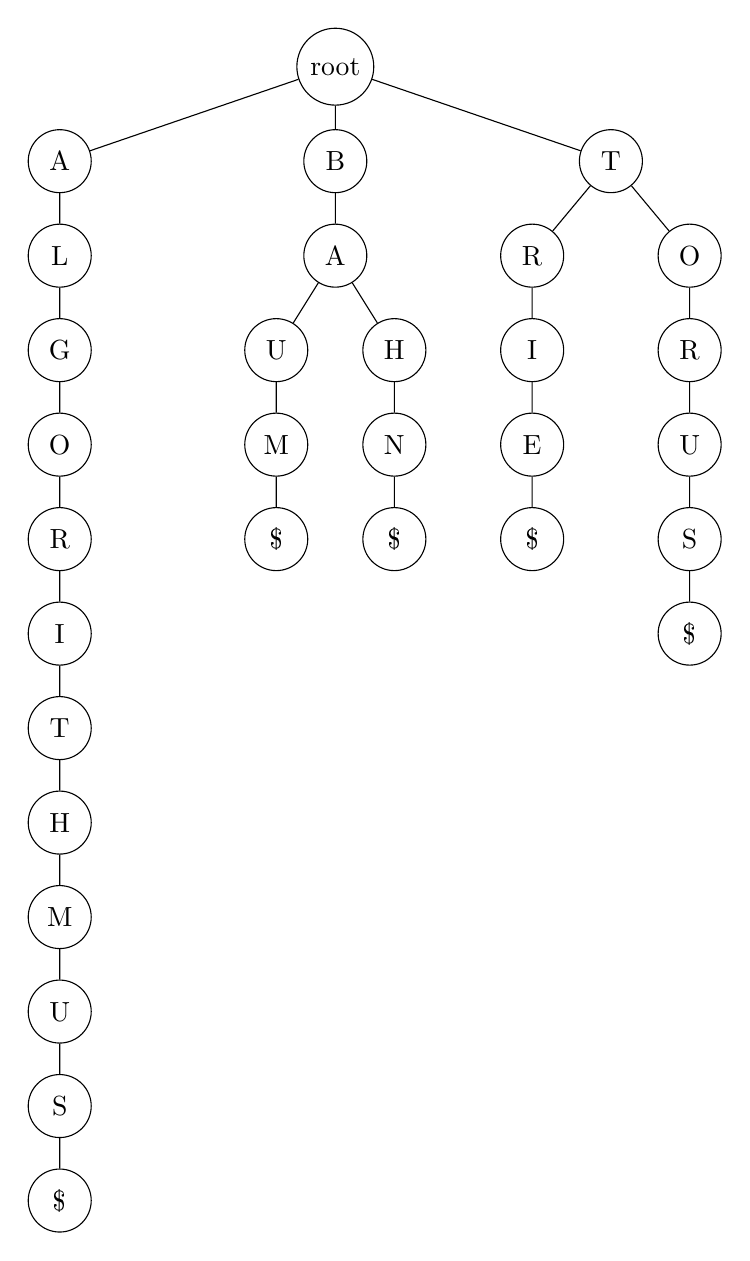
\begin{tikzpicture}[
  level distance=1.2cm,
  level 1/.style={sibling distance=3.5cm},
  level 2/.style={sibling distance=2cm},
  level 3/.style={sibling distance=1.5cm},
  every node/.style={draw, circle, minimum size=0.8cm}
]

\node {root}
  child {node {A}
    child {node {L}
      child {node {G}
        child {node {O}
          child {node {R}
            child {node {I}
              child {node {T}
                child {node {H}
                  child {node {M}
                    child {node {U}
                      child {node {S}
                        child {node {\$}}
                      }
                    }
                  }
                }
              }
            }
          }
        }
      }
    }
  }
  child {node {B}
    child {node {A}
      child {node {U}
        child {node {M}
          child {node {\$}}
        }
      }
      child {node {H}
        child {node {N}
          child {node {\$}}
        }
      }
    }
  }
  child {node {T}
    child {node {R}
      child {node {I}
        child {node {E}
          child {node {\$}}
        }
      }
    }
    child {node {O}
      child {node {R}
        child {node {U}
          child {node {S}
            child {node {\$}}
          }
        }
      }
    }
  };
\end{tikzpicture}

\newpage

\begin{center}
    \textbf{6. insert(TORPEDO)}
\end{center}
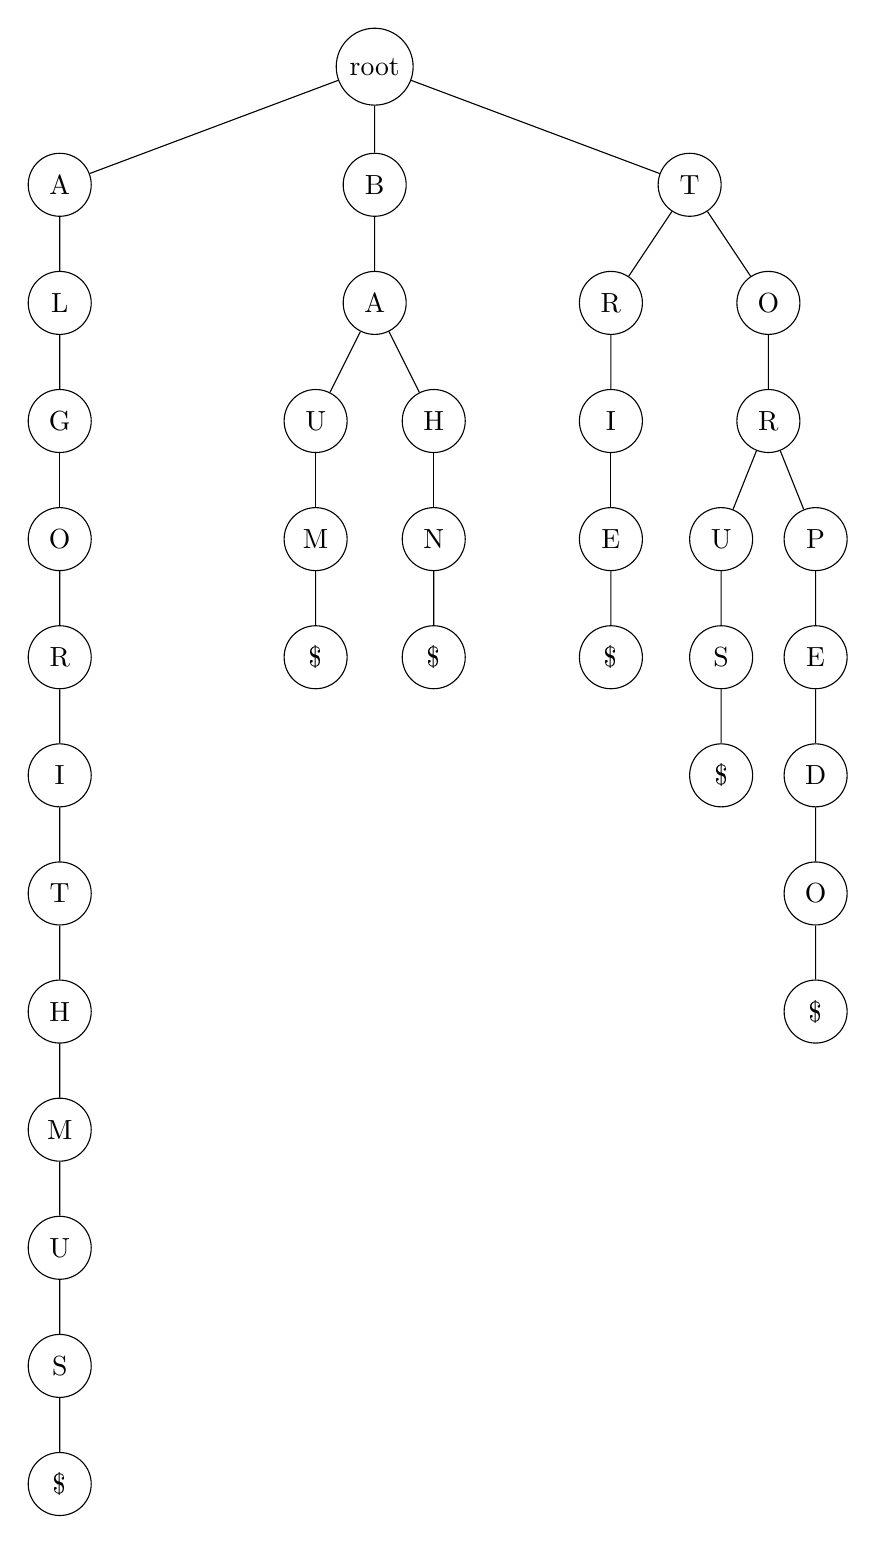
\begin{tikzpicture}[
  level distance=1.5cm,
  level 1/.style={sibling distance=4cm},
  level 2/.style={sibling distance=2cm},
  level 3/.style={sibling distance=1.5cm},
  level 4/.style={sibling distance=1.2cm},
  level 5/.style={sibling distance=1cm},
  every node/.style={draw, circle, minimum size=0.8cm}
]

\node {root}
  child {node {A}
    child {node {L}
      child {node {G}
        child {node {O}
          child {node {R}
            child {node {I}
              child {node {T}
                child {node {H}
                  child {node {M}
                    child {node {U}
                      child {node {S}
                        child {node {\$}}
                      }
                    }
                  }
                }
              }
            }
          }
        }
      }
    }
  }
  child {node {B}
    child {node {A}
      child {node {U}
        child {node {M}
          child {node {\$}}
        }
      }
      child {node {H}
        child {node {N}
          child {node {\$}}
        }
      }
    }
  }
  child {node {T}
    child {node {R}
      child {node {I}
        child {node {E}
          child {node {\$}}
        }
      }
    }
    child {node {O}
      child {node {R}
        child {node {U}
          child {node {S}
            child {node {\$}}
          }
        }
        child {node {P}
          child {node {E}
            child {node {D}
              child {node {O}
                child {node {\$}}
              }
            }
          }
        }
      }
    }
  };
\end{tikzpicture}

\newpage

\textbf{komprimierten Trie:}

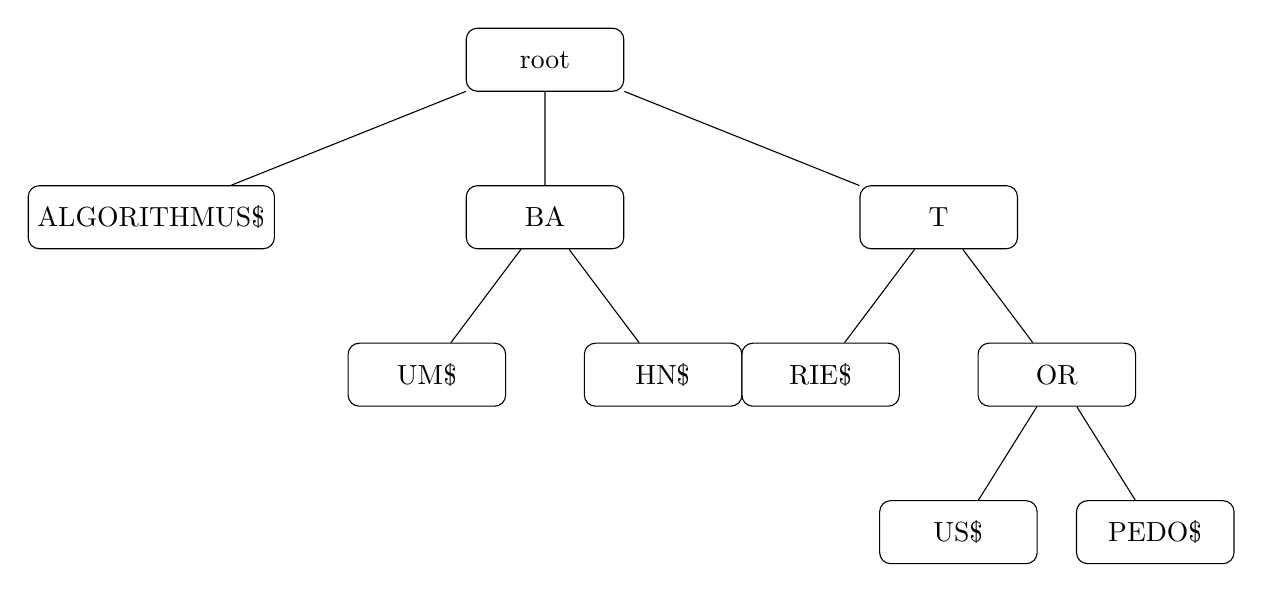
\begin{tikzpicture}[
  level distance=2cm,
  level 1/.style={sibling distance=5cm},
  level 2/.style={sibling distance=3cm},
  level 3/.style={sibling distance=2.5cm},
  every node/.style={draw, rectangle, rounded corners, minimum height=0.8cm, minimum width=2cm, align=center}
]

\node {root}
  child {node {ALGORITHMUS\$}}
  child {node {BA}
    child {node {UM\$}}
    child {node {HN\$}}
  }
  child {node {T}
    child {node {RIE\$}}
    child {node {OR}
      child {node {US\$}}
      child {node {PEDO\$}}
    }
  };
\end{tikzpicture}

\vspace{1cm}
\begin{center}
\small\textit{Enthält die Wörter: ALGORITHMUS, TRIE, BAUM, TORUS, BAHN, TORPEDO}
\end{center}





\noindent
\textbf{b)} Entwickeln Sie einen Algorithmus, der alle Wörter in einem unkomprimierten Trie ausgibt und dabei jede Kante höchstens zweimal besucht.\\